% %%%%%%%%%%%%%%%%%%%%%%%%%%%%%%%%%%%%%%%%%%%%%%%%%%%%%%%%%%%%%%%%%%%%%%%%%%%%%
% %%%%%%%%%%%%%%%%%%%%%%%%%%%%%%%%%%%%%%%%%%%%%% Description of Numerical Model
% %%%%%%%%%%%%%%%%%%%%%%%%%%%%%%%%%%%%%%%%%%%%%%%%%%%%%%%%%%%%%%%%%%%%%%%%%%%%%

\chapter{Numerical Model}
\label{ch_model}

The model works in two and a half dimensions. A meridional slice of the magnetosphere is resolved. Fields are presumed to vary azimuthally according to a fixed modenumber \azm. Derivatives in $\phi$ are replaced by $i \azm$. Imaginary field values indicate a phase shift in the azimuthal direction. 

\todo{Note that Lysak's 2013 paper\cite{lysak_2013} was 2.5D. }

The use of a fixed modenumber allows a dramatic decrease in computational cost. Waves with very high azimuthal modenumber are prohibitively expensive to simulate since they can only be resolved if grid resolution is very fine in the azimuthal direction. 

\todo{Has anyone actually talked about computational expense as a constraint on high-\azm simulations?}

This prevents the simultaneous consideration of dayside and nightside phenomena, but is fine for azimuthally-localized waves. As was shown by \cite{engebretson_1987}, and recently confirmed in detail by \cite{dai_2015}, Pc4 pulsations are generally confined to just a few hours MLT on the dayside. 

Driving with a compressional pulse from the outer boundary of a simulation is typical. This model also includes a novel driving mechanism: perturbations to the ring current. 

The code is linear. All magnetic fields are a first-order perturbation over the zeroth-order dipole field. This is a not-great assumption out towards the magnetopause. In practice, however, most activity is within $L \sim \SI{7}{\RE}$, where the dipole approximation is pretty good. 

Models with height-resolved ionospheres are a very recent development. Lysak presented his in 2013\cite{lysak_2013}. 

Ground signatures are fairly recent as well. 

\todo{Some ground signature work as far back as Greifinger and Greifinger in 1968, but there's been steady advancement. Lysak and Song, in 2006, were the first to work out ground signatures without the assumption of a single-frequency wave. }

\todo{The support software -- the driver and the plotter -- are significant too. Do they go in a section? In an appendix? }

\todo{Past FLR simulations focused on a single mode, didn't account well for the ionosphere, etc. Lee and Lysak 1989, 1990, 1991, Rankin et al 1993, 1995, 1999, Tikhonchuk and Rankin 2000, 2002. }

\todo{Past work that got ground signatures (without latitude-dependent zenith angle) Greifinger and Greifinger 1968, 1973, Hughes 1974, Sciffer and Waters 2002, Sciffer et al 2005. Better computation of ground signatures... Waters and Sciffer 2008, Sciffer and Waters 2011, Woodroffe and Lysak 2012. }

Note that the model uses \si{\mega\meter}, \si{\second}, \si{\mega\coulomb}, and \si{\gram} as the fundamental units of length, time, charge, and mass respectively. As a result, electric field is measured in \si{\mV/\meter}, magnetic field is measured in \si{\nano\tesla}, and Poynting flux is measured in \si{\mW/\meter\squared}. 



% =============================================================================
% =============================================================================
% =============================================================================
\section{Coordinate System}
  \label{sec_coords}

When referring to fields in place, it's convenient to use lowercase\footnote{ Not to be confused with uppercase \X, \Y, and \Z, which orient relative to the sun; see \cref{ch_intro} } \x, \y, and \z in their usual dipolar sense. The unit vector \zhat is aligned with the dipole field (pointing outward in the northern hemisphere and inward in the southern hemisphere), while \xhat is perpendicular to \zhat within the meridional plane and \yhat points in the azimuthal direction. 

\todo{Double-check the signs for \x (radially inward or outward at the equator?) and \y (east or west?). }

\todo{Wait... are \x, \y, and \z the same as Radoski's coordinates? }

It's convenient to align the grid with the zeroth-order magnetic field, which is presumed to be a perfect dipole. Field line resonances (such as Pc4 pulsations) are guided by magnetic field lines. 

\todo{Who showed that ULF waves can be guided? Cite them. }

\todo{Discuss, in Future Work, how the grid would be generalized. }

Radoski did theoretical work in the following dipole coordinates\cite{radoski_1967_coords}. 
\begin{align}
  \label{radoski_coords}
  \radx & = -\frac{\sin^2 \theta}{r} & \rady & = \phi & \radz & = \frac{\cos \theta}{r^2}
\end{align}

\todo{The symbol $\nu$ is overused. Reserve it for collision frequency. Use something else here. }

It's also convenient to take into account the effects of the ionosphere, the lower boundary of which is governed by gravity, and thus has a more-or-less constant altitude. If the above coordinates are used, no line of constant $\radz$ coincides with the ionosphere, at least not over a significant range of latitudes. 

Many previous works have used an effective ionosphere of nonuniform altitude. 

\todo{Figure out which previous works are worth citing here. Options include Radoski 1967, Lee and Lysak 1989, 1991, Rankin et al 1993, 1994, Streltsov and Lotko 1995, 1999. }


\todo{"The ionosphere is important for \Alfven waves." Cite this. }

In order to accommodate dipole field lines as well as a fixed-altitude ionosphere, a nonorthogonal grid is necessary. Such a grid was worked out numerically by Proehl\cite{proehl_2002}, then formalized analytically by Lysak\cite{lysak_2004}:
\begin{align}
  \label{def_coords}
  \lysakx & = - \frac{R_I}{r} \sin^2 \theta & 
  \lysaky & = \phi &
  \lysakz & = \frac{R_I^2}{r^2} \frac{\cos \theta}{\cos \theta_0}
\end{align}

The term $R_I$ indicates the ionosphere's position relative to Earth's center. It's generally taken to be \SI{1}{\RE} + \SI{100}{\km}. 

Like \radx and \rady, the coordinates \lysakx and \lysaky index a field line. However, compared to \radz, \lysakz has been renormalized by $\cos \theta_0$, where $\theta_0$ is the colatitude where each field line intersects the ionosphere in the northern hemisphere. As a result, for all field lines, $\lysakz = \pm 1$ at the northern and southern foot points. 

In terms of the McIlwain parameter, $\lysakx = -\frac{R_I}{L}$, and $\cos \theta_0 = \sqrt{ 1 - \frac{R_I}{L} }$

Compared to \cref{radoski_coords}, \cref{def_coords} represents a renormalization of indexing along each field line. The field lines themselves are not deformed. 

\todo{Explain how we set up the grid. It should only take a paragraph or two -- it doesn't need its own section. }

\todo{Plot of the grid setup! }

% -----------------------------------------------------------------------------
% -----------------------------------------------------------------------------
% -----------------------------------------------------------------------------
\subsection{Covariant and Contravariant Bases}
  \label{sec_basis}

The coordinates defined in \cref{def_coords} are not orthonormal. As a result, it's necessary to consider covariant and contravariant basis vectors separately. 

Covariant basis vectors $e_i \equiv \dd{\lysaki} \vec{x}$ are normal to the curve defined by constant $\lysaki$. 

Contravariant basis vectors $e^i \equiv \dd{ \vec{x} } \lysaki$ are tangent to the coordinate curve. Equally, they're normal to the plane defined by constant $\lysakj$ for all $j \ne i$. 

The basis vectors are reciprocal to one another\cite{dhaeseleer_1991}, and can be used to define the metric tensor $g$. 
\begin{align}
  \label{metric_basics}
  \hat{e}^i \cdot \hat{e}_j &= \delta^i_j & \hat{e}_i \cdot \hat{e}_j &= g_{ij} & \hat{e}^i \cdot \hat{e}^j &= g^{ij}
\end{align}

Note $\delta^i_j$ is the Kronecker delta, $\varepsilon^{ijk}$ is the Levi-Civita symbol, and summation is implied over repeated indeces per Einstein's convention\cite{einstein_1916}. 

The metric tensor is used to map between the covariant and contravariant representations of a vector
\begin{align}
  \label{metric_usage}
  A_i &= g_{ij} A^j & A^i &= g^{ij} A_j && \text{where} & A_i &\equiv \vec{A} \cdot \hat{e}_i &  A^i &\equiv \vec{A} \cdot \hat{e}^i
\end{align}

The Jacobian, used for mapping differential volume elements between bases, can be expressed as the square root of the determinant of the metric tensor. 
\begin{align}
  \label{def_jacobian}
  \jac &= \sqrt{ \varepsilon^{ijk} g_{1i} g_{2j} g_{3k} } && \text{where} & \jac d\lysakx d\lysaky d\lysakz &= dV
\end{align}

This quantity is also used when expressing a curl or cross product in generalized coordinates. 
\begin{align}
  \label{jacobian_usage}
  \lr{ \curl{A} }^i &= \frac{ \varepsilon^{ijk} }{\jac} \dd{\lysakj} A_k & \lr{ \cross{A}{B} }^i &= \frac{ \varepsilon^{ijk} }{\jac} A_j B_k
\end{align}

% -----------------------------------------------------------------------------
% -----------------------------------------------------------------------------
% -----------------------------------------------------------------------------
\subsection{Mapping to Physical Coordinates}

The full expression for the basis vectors, metric tensor, and Jacobian determinant discussed in \cref{sec_basis} can be found in the appendix of \cite{lysak_2004}. 

\todo{These expressions should probably be written out an in appendix here too...}

The basis vectors can be renormalized to produce unit vectors along the dipole coordinates \x, \y, and \z. 
\begin{align}
  \label{def_xyz_directions}
  \xhat &= \frac{1}{ \sqrt{ g^{11} } } \hat{e}^1 &
  \yhat &= \frac{1}{ \sqrt{ g^{22} } } \hat{e}^2 &
  \zhat &= \frac{1}{ \sqrt{ g_{33} } } \hat{e}_3
\end{align}

In addition, this coordinate system provides horizontal and radial unit vectors. Note that \cref{def_rqf_directions} is valid only at the ionospheric boundary. 
\begin{align}
  \label{def_rqf_directions}
  \qhat &= \frac{1}{ \sqrt{ g_{11} } } \hat{e}_1 &
  \fhat &= \frac{1}{ \sqrt{ g_{22} } } \hat{e}_2 &
  \rhat &= \frac{1}{ \sqrt{ g^{33} } } \hat{e}^3
\end{align}

% =============================================================================
% =============================================================================
% =============================================================================
\section{Ionospheric Profile}
  \label{sec_ionos}

The ionospheric profiles used in this model are based on values tabulated in the Appendix B of Kelley's book\cite{kelley_1989}. They were adapted by Lysak\cite{lysak_2013} to take into account the effect of the magnetosphere's latitude-dependent density profile. 

Mean molecular mass of \SI{28}{\amu} at \SI{100}{\km}, \SI{16}{\amu} around \SI{400}{\km}, down to \SI{1}{\amu} above \SI{1400}{\km}. 

Simulations are carried out using four profiles: active day, quiet day, active night, quiet night. 

Profiles are static for the duration of a simulation. Even so-called ultra low frequency waves are still much faster than convective timescales. 

\todo{Come up with a characteristic convective timescale or two, and cite it. }

% -----------------------------------------------------------------------------
% -----------------------------------------------------------------------------
% -----------------------------------------------------------------------------
\subsection{Conductivity}

The conductivity profiles used in this model are the tabulated values from \cite{kelley_1989}, rescaled by Lysak\cite{lysak_2013} to account for the increased mean molecular mass at low altitudes. 
\begin{align}
  \sp &= \displaystyle\sum_s \frac{n_s q_s^2}{m_s} \frac{\nu_s}{\nu_s^2 + \Omega_s^2} &
  \sh &= -\displaystyle\sum_s \frac{n_s q_s^2}{m_s} \frac{\Omega_s}{\nu_s^2 + \Omega_s^2} &
  \sz &= \displaystyle\sum_s \frac{n_s q_s^2}{m_s \nu_s}
\end{align}

Each profile is resolved to an altitude of about $\SI{1e4}{\km}$, and include well-resolved $E$, $F_1$, and $F_2$ layers. 

\todo{Talk about the ionospheric layers, probably in the introduction. }

\begin{figure}[H]
    \centering
    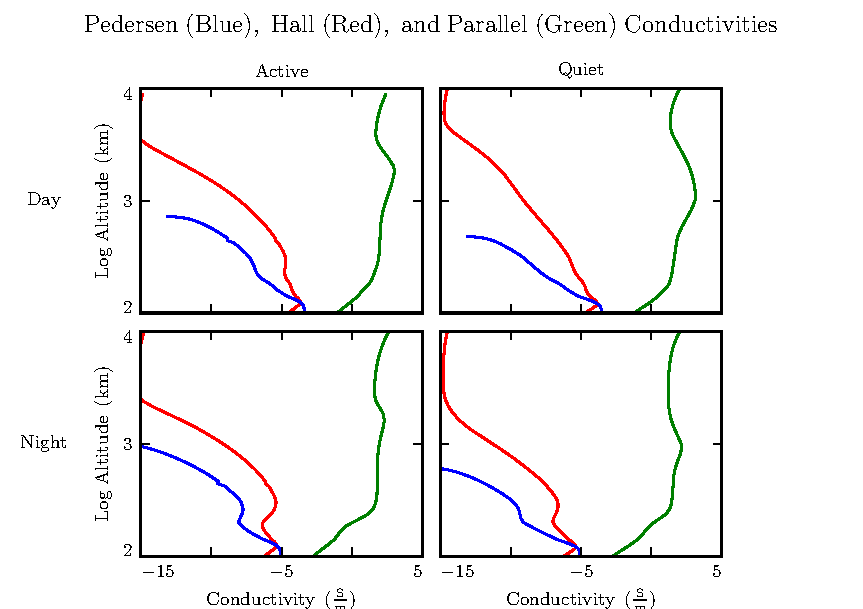
\includegraphics[width=\textwidth]{figures/sigma.pdf}
    \caption[Ionospheric Conductivity Profiles]{
      Ionospheric conductivity profiles, adapted by Lysak\cite{lysak_2013} from Appendix B of Kelley's textbook\cite{kelley_1989}. 
    }
    \label{fig_sigma}
\end{figure}

% -----------------------------------------------------------------------------
% -----------------------------------------------------------------------------
% -----------------------------------------------------------------------------
\subsection{\Alfven Speed}

The \Alfven speed is computed from Kelley's low-density profile, modified to take into account the local density. The density, in turn, is the sum of a plasmaspheric profile and a high-latitude auroral profile. 
\begin{align}
  \ep &= \text{(low-density tabulated value)} + \frac{ n \bar{m} }{B_0^2}
\end{align}

\todo{What's a clean way of showing the low-density \ep that we read in? }

\todo{Above the profile, Bob scales the value that's read in as $r^5$ or something. Is there a citation for that? }

Where $\bar{m}$ is the ambient mean molecular mass and $B_0$ is the zeroth-order magnetic field strength, $B_0 = \SI{3.11e4}{\nano\tesla} \lr{ \frac{R_E}{r} }^3 \sqrt{ 1 + 3 \cos^2 \theta }$. Note that \SI{3.11e4}{\nano\tesla} is the value of the Earth's magnetic field at the equator on Earth's surface. 

\todo{Cite this number? }

Note that we do not scale the electric constant to units of $\ez$. 

The \Alfven speed is then computed per \cref{def_basics}, $\va^2 \equiv \frac{1}{\mz \ep}$. 

\todo{Put up a plot of the four \Alfven speed profiles. Show the dipole, or zoom in on the ionosphere? }

\todo{Shouldn't the \Alfven speed profiles be brought up early on, since they're necessary for discussions about evanescence at large \azm in \cref{ch_math}? }

\todo{Explain in this section how we figure out the time step. }

% =============================================================================
% =============================================================================
% =============================================================================
\section{Maxwell's Equations}
  \label{sec_eqns}

The model simulates the evolution of electric and magnetic fields in accordance with Maxwell's equations. Specifically, magnetic fields are advanced using \farlaw, and electric fields with \amplaw. Kirchhoff's formulation of \ohmlaw ($\vec{J} = \tensor{\sigma} \cdot \vec{E}$) is used to eliminate the explicit current dependence in \amplaw. 
\begin{align}
  \label{def_eqns}
  \ddt \vec{B} &= - \curl{E} &
  \tensor{\epsilon} \cdot \ddt \vec{E} &= \frac{1}{\mu_0} \curl{B} - \tensor{\sigma} \cdot \vec{E}
\end{align}

% -----------------------------------------------------------------------------
% -----------------------------------------------------------------------------
% -----------------------------------------------------------------------------
\subsection{Notation and Optimization}

Algebra is carried out on paper, producing expressions where each field value is a linear combination of previous field values. These coefficients are computed before the main loop begins. This offers a significant reduction in floating point operations each iteration. 

The \assign operator is used to indicate assignment, rather than equality. Values on the left are new, and those on the right are old. New and old magnetic field values are offset by \dt; electric field values staggered by $\frac{\dt}{2}$. As an example of this notation, \cref{def_assign} integrates \farlaw over a time step, assuming that the curl of the electric field varies slowly compared to \dt: 
\begin{align}
  \label{def_assign}
  \begin{split}
  \int_0^{\dt} dt \, \ddt \vec{B} &= - \displaystyle\int_0^{\dt} dt \, \curl{E} \\ 
  \left. \vec{B} \right|_{\dt} - \left. \vec{B} \right|_0 &= \left. - \dt \, \curl{E} \right|_{ \frac{\dt}{2} } \\
  \vec{B} &\assign \vec{B} - \dt \, \curl{E}
  \end{split}
\end{align}

It's also beneficial to store the curl of each field, rather than take derivatives on the fly. The following sections make use of the shorthand $\vec{C} \equiv \curl{E}$ and $\vec{F} \equiv \curl{B}$. Or, recalling \cref{jacobian_usage}, 
\begin{align}
  \label{def_curls}
  C^i & = \frac{ \varepsilon^{ijk} }{\jac} \dd{\lysakj} E_k &
  F^i & = \frac{ \varepsilon^{ijk} }{\jac} \dd{\lysakj} B_k
\end{align}

Only covariant field components are stored. Only contravariant curl components are stored. This cuts down on memory use, while also eliminating the time spent rotating between bases; those operations are built into the precomputed coefficients. 

% -----------------------------------------------------------------------------
% -----------------------------------------------------------------------------
% -----------------------------------------------------------------------------
\subsection{Magnetic Fields}

Taking advantage of the shorthand defined in \cref{def_curls}, \farlaw is simply written
\begin{align}
  \label{farlaw_ijk}
  \ddt B^i &= - C^i
\end{align}

Or, using the metric tensor to cast the magnetic field in terms of its covariant components, and writing out each coefficient explicitly,
\begin{align}
  \begin{split}
  B_1 &\assign B_1 - g_{11} \, \dt \, C^1 - g_{13} \, \dt \, C^3 \\
  B_2 &\assign B_2 - g_{22} \, \dt \, C^2 \\
  B_3 &\assign B_3 - g_{31} \, \dt \, C^1 - g_{33} \, \dt \, C^3
  \end{split}
\end{align}


% -----------------------------------------------------------------------------
% -----------------------------------------------------------------------------
% -----------------------------------------------------------------------------
\subsection{Electric Fields}

\amplaw, can be solved with integrating factors. From \cref{def_eqns}, 
\begin{align}
  \tensor{\epsilon} \cdot \ddt \vec{E} &= \frac{1}{\mu_0} \curl{B} - \tensor{\sigma} \cdot \vec{E}
\end{align}

The permittivity tensor is diagonal, and so can be trivially inverted. 
\begin{align}
  \label{amp_tensor}
  \lr{ \tensor{\Omega} + \tensor{ \mathbb{I} } \ddt } \cdot \vec{E} &= \tensor{v}^2 \cdot \vec{F}
\end{align}

Where $\tensor{ \mathbb{I} }$ is the identity tensor and in \x-\y-\z coordinates, 
\begin{align}
  \tensor{v}^2 &\equiv \frac{1}{\mz} \tensor{\epsilon}^{-1} = 
    \mmm{\va^2}{0}{0}
        {0}{\va^2}{0}
        {0}{0}{c^2}
  && \text{and} &
  \tensor{\Omega} &\equiv \tensor{\epsilon}^{-1} \cdot \tensor{\sigma} = 
    \mmm{ \frac{\sp}{\ep} }{ -\frac{\sh}{\ep} }{0}
        { \frac{\sh}{\ep} }{ \frac{\sp}{\ep} }{0}
        {0}{0}{ \frac{\sz}{\ez} } 
\end{align}

Using integrating factors, \cref{amp_tensor} gives
\begin{align}
  \vec{E} &\assign \exp \arg{ -\tensor{\Omega} \; \dt } \cdot \vec{E} + \dt \, \tensor{v}^2 \cdot \exp \arg{ -\tensor{\Omega} \; \tfrac{\dt}{2} } \cdot \vec{F}
\end{align}

\todo{Do we need to be careful here about the difference between a matrix and a tensor? }

The tensor exponential can be evaluated by considering the diagonal and off-diagonal terms separately. 
\begin{align}
  \tensor{\Omega} &= \tensor{\Omega}'
    + \frac{\sh}{\ep} 
    \mmm{0}{-1}{0}
        {1}{0}{0}
        {0}{0}{0} && \text{where} &
  \tensor{\Omega}' &=
    \mmm{ \frac{\sp}{\ep} }{0}{0}
        {0}{ \frac{\sp}{\ep} }{0}
        {0}{0}{ \frac{\sz}{\ez} }
\end{align}

Note that tensors are remarkably well-behaved when exponentiated\cite{hall_2015}, particularly since $\tensor{\Omega}'$ is diagonal, and thus they commute. 
\begin{align}
  \exp \arg{ \tensor{T} } &= \displaystyle\sum_n \frac{1}{ n! } \tensor{T}^n && \text{and} & \exp \arg{ \tensor{T} + \tensor{T}' } &= \exp \arg{ \tensor{T} } \exp \arg{ \tensor{T}' }
\end{align}

The off-diagonal terms collapse into sines and cosines, indicating a rotation about \z. 
\begin{align}
  \label{amp_final}
  \vec{E} &\assign \exp \arg{ -\tensor{\Omega}' \; \dt } \cdot \tensor{R}_z \arg{ \tfrac{-\sh \dt}{\ep} } \cdot \vec{E}
   + \dt \, \tensor{v}^2 \cdot \exp \arg{ -\tensor{\Omega}' \; \tfrac{\dt}{2} } \cdot \tensor{R}_z \arg{ \tfrac{-\sh \dt}{2 \ep} } \cdot \vec{F}
\end{align}

Where 
\begin{align}
  \tensor{R}_z \arg{\theta} &= 
  \mmm{\cos\theta}{-\sin\theta}{0}
      {\sin\theta}{\cos\theta}{0}
      {0}{0}{1}
\end{align}

The parallel term of term of \cref{amp_final} is simply
\begin{align}
  \label{amp_para}
  E_\parallel \assign E_\parallel \exp \arg{ \tfrac{- \sz \dt}{\ez} } + c^2 \dt F_\parallel \exp \arg{ \tfrac{- \sz \dt}{2 \ez} }
\end{align}

For the aforementioned ionospheric profiles and time steps, $\frac{\sz \dt}{\ez}$ is never smaller than $10^3$. As a result, $\exp \arg{ - \frac{\sz \dt}{\ez} }$ is far too small to be stored in a double precision variable. That is, this simulation takes $E_\parallel$ (and, equally, $E_3$) to be uniformly zero. 

This, obviously, precludes any discussion of parallel electric fields or parallel currents. These topics are revisited in \cref{ch_inertia}. 

Not unrelatedly, recalling the definition of the plasma frequency and parallel conductivity from \cref{def_basics}, $\frac{\sz}{\ez}$ can also be written $\frac{\op^2}{\nu}$. 

The plasma frequency is very fast. 

The perpendicular components of \cref{amp_final}, mapped from the physical basis to the contravariant basis (per \cref{def_xyz_directions}) to the covariant basis (per \cref{metric_usage}), give
\begin{alignat}{6}
  \label{e1_final}
  & E_1 + \frac{ g^{13} }{ g^{11} } && E_3 \assign &&   && E_1 && \cos \arg{ \tfrac{- \sh \dt}{\ep} } \exp \arg{ \tfrac{- \sp \dt}{\ep} } &&  \notag \\
  &                                 &&             && + && E_2 && \sin \arg{ \tfrac{- \sh \dt}{\ep} } \exp \arg{ \tfrac{- \sp \dt}{\ep} } &&  \sqrt{ \frac{ g^{22} }{ g^{11} } } \notag \\
  &                                 &&             && + && E_3 && \cos \arg{ \tfrac{- \sh \dt}{\ep} } \exp \arg{ \tfrac{- \sp \dt}{\ep} } &&  \frac{ g^{13} }{ g^{11} } \\
  &                                 &&             && + && F^1 && \cos \arg{ \tfrac{- \sh \dt}{2\ep} } \exp \arg{ \tfrac{- \sp \dt}{2\ep} } &&  \frac{\va^2 \dt}{ g^{11} } \notag \\
  &                                 &&             && + && F^2 && \sin \arg{ \tfrac{- \sh \dt}{2\ep} } \exp \arg{ \tfrac{- \sp \dt}{2\ep} } &&  \frac{\va^2 \dt}{ \sqrt{ g^{11} g^{22} } } \notag \\
  \intertext{and}
  \label{e2_final}
  & && E_2 \assign && - && E_1 && \sin \arg{ \tfrac{- \sh \dt}{\ep} } \exp \arg{ \tfrac{- \sp \dt}{\ep} } &&  \sqrt{ \frac{ g^{11} }{ g^{22} } } \notag \\
  & &&             && + && E_2 && \cos \arg{ \tfrac{- \sh \dt}{\ep} } \exp \arg{ \tfrac{- \sp \dt}{\ep} } &&  \notag \\
  & &&             && - && E_3 && \sin \arg{ \tfrac{- \sh \dt}{\ep} } \exp \arg{ \tfrac{- \sp \dt}{\ep} } &&  \frac{ g^{13} }{ \sqrt{ g^{11} g^{22} } } \\
  & &&             && - && F^1 && \sin \arg{ \tfrac{- \sh \dt}{2\ep} } \exp \arg{ \tfrac{- \sp \dt}{2\ep} } &&  \frac{\va^2 \dt}{ \sqrt{ g^{11} g^{22} } } \notag \\
  & &&             && + && F^2 && \cos \arg{ \tfrac{- \sh \dt}{2\ep} } \exp \arg{ \tfrac{- \sp \dt}{2\ep} } &&  \frac{\va^2 \dt}{ g^{22} } \notag
\end{alignat}

The $E_3$ terms can be ignored at present, but \cref{ch_inertia} references back to them. 


% =============================================================================
% =============================================================================
% =============================================================================
\section{Driving}
  \label{sec_driving}

If no energy is added, the simulation is pretty boring. Everything just stays zero. 

% -----------------------------------------------------------------------------
% -----------------------------------------------------------------------------
% -----------------------------------------------------------------------------
\subsection{Outer Boundary Compression}

Driving from the outer boundary is the traditional way to do it. 

\todo{Cite and briefly explain past work done with compressional driving. This is what most of Bob's papers are, right? }

As discussed in \cref{sec_math_implications}, \Alfven waves become guided when the azimuthal modenumber is large. The energy all stays close to the outer boundary. No field line resonances of significant strength are created within the magnetosphere. 

\todo{Show a plot of compressional driving, maybe day and night, as \azm increases. Mean energy density over time? Something that shows the recession of waves away from the middle of the simulation. }

Compressional driving is applied by setting the value of $B_3$ at the outer boundary. 

% -----------------------------------------------------------------------------
% -----------------------------------------------------------------------------
% -----------------------------------------------------------------------------
\subsection{Ring Current Modulation}

Pc4 pulsations with high azimuthal modenumber are known to be driven from within the magnetosphere, such as through drift-resonant interactions with energetic radiation belt and ring current particles. 

\todo{Cite. }

Substorm injection can cause localized ring current behavior. 

\todo{UNH was looking at this at AGU. Check if they have published yet. }

During geomagnetically active times, the ring current is a dynamic region. It's easy to imagine localized perturbations. 

It's difficult to estimate how large such perturbations might be. The following is a kludgey estimate. 

\todo{Plot of Sym-H and its Fourier modes. }

The noise suggests that a Fourier component with a period of about \SI{1}{\minute} could have an amplitude around \SI{e-3}{\nano\tesla}. 

If the driving is delivered at $L=5$, with a standard deviation of \SI{0.5}{\RE} in the radial direction and \SI{5}{\degree} angularly, that corresponds to a current density of about \SI{4e-4}{\uA/\meter\squared}. 

\todo{What electric field magnitude does this correspond to? }

Current driving is applied by adding an additional current term. \amplaw becomes
\begin{align}
  \tensor{\epsilon} \cdot \ddt \vec{E} &= \frac{1}{\mu_0} \curl{B} - \tensor{\sigma} \cdot \vec{E} - \vec{J}_{drive}
\end{align}

And this driving term is absorbed into the curl by revising \cref{def_curls} from $\vec{F} \equiv \curl{B}$ to $\vec{F} \equiv \curl{B} - \vec{J}_{drive}$. (As a result, \cref{e1_final,e2_final} do not change.)




... \\

... \\

... \\





%\begin{align}
%  \label{amp_perp}
%  \ep \ddt \vec{E}_\bot &= \frac{1}{\mu_0} \lr{ \curl{B} }_\bot - \tensor{\sigma}_\bot \cdot \vec{E}_\bot
%\end{align}

%Cast in terms of the linear polarizations $E_x$ and $E_y$, this is a pair of coupled differential equations. However, in a circularly-polarized basis, the conductivity tensor is diagonal. Taking $E_\pm \equiv \frac{1}{ \sqrt{2} } \lr{E_x \pm i E_y}$, and defining components of \curl{B} analogously, \cref{amp_perp} can be written
%\begin{align}
%  \ep \ddt E_\pm &= \frac{1}{\mu_0} \lr{ \curl{B} }_\pm - \lr{ \sp \pm i \sh } E_\pm
%\end{align}

%Using integrating factors, and recalling $\va^2 \equiv \frac{1}{\mu_0 \ep}$, the new values of $E_\pm$ can be separated from the old. 
%\begin{align}
%  E_\pm &\assign E_\pm \exp \arg{- \tfrac{\sp \pm i \sh}{\ep} \dt} + \va^2 \dt \lr{ \curl{B} }_\pm \exp \arg{ - \tfrac{\sp \pm i \sh}{\ep} \tfrac{\dt}{2} }
%\end{align}

%Rotating from circular polarization to linear causes the imaginary terms within each exponential to cancel out, leaving sines and cosines. The expression can then be written
%\begin{align}
%  \label{eperp_tensor}
%  \vec{E}_\bot &\assign 
%  \tensor{R} \arg{ \tfrac{- \sh \dt}{\ep} } \cdot
%  \vec{E}_\bot \exp \arg{ \tfrac{- \sp \dt}{\ep} } +
%  \va^2 \dt \tensor{R} \arg{ \tfrac{- \sh \dt}{2 \ep} } \cdot
%  \lr{ \curl{B} }_\bot \exp \arg{ \tfrac{- \sp \dt}{2 \ep} }
%\end{align}

%Where $\tensor{R}$ is the rotation matrix
%\begin{align}
%  \tensor{R} \arg{\theta} \equiv \mm{\cos\theta}{-\sin\theta}{\sin\theta}{\cos\theta}
%\end{align}


We look at Sym-H to get an idea of the appropriate scale for current driving. We look at a few storms. 1 June 2013. 17 March 2015. 22 June 2015. 17 March 2013. A few in October and November 2012. 

We plot the power spectrum and basically do a fit for the top of the range of $\frac{1}{f}$ noise. This gives us a typical magnitude for oscillations on the order of a minute. 

This doesn't give us a characteristic spatial extent for ring current modulations -- Sym-H is a global index -- but we can eyeball the size of current fluctuations. We know the approximate size of the ring current, so we can go from ground-based field signature to current density in space pretty easily. 

There are a lot of parameters to play with. Since this is a linear code, we don't have to worry about ``sweet spots'' for nonlinear effects in the driving magnitude. And it doesn't look like the exact position or shape of the ring current has much qualitative effect on what we see. 

Looking at SYMH. Fourier series out to a period of about a minute. The power spectrum (judging from June 1-3 2013) gives you ~$10^{-2} (T/minutes)$. We can hand-wave a mapping from SYMH to the ring current. 
\begin{align}
  B & = \frac{\mu_0 I}{2 R}
\end{align}

With $B \sim \SI{2}{\nano\tesla}$, $R \sim \SI{4}{\RE}$, $A \sim \SI{1}{\RE\squared}$, we end up with $J \sim \SI{e-4}{\micro\ampere/\meter\squared}$. 

% =============================================================================
% =============================================================================
% =============================================================================
\section{Boundary Conditions}
  \label{sec_bcs}


The grid can't go on forever. There have to be special cases at the edges. 

% -----------------------------------------------------------------------------
% -----------------------------------------------------------------------------
% -----------------------------------------------------------------------------
\subsection{Parity and Interpolation}

At the inner and outer boundaries (that is, along the innermost and outermost field lines), as use Dirichlet and Neumann boundary conditions for electric and magnetic fields respectively. 

These are implemented in the differentiation and (parity) interpolation functions. 

Whenever we need to know the magnetic field just outside the grid boundary, we say that its value is the same as just inside the grid boundary, and its derivative is zero. Neumann. 

Conversely, we say that the electric field just outside the grid goes to 0, allowing us to compute the derivative from the value just inside the grid. Dirichlet. 

Dirichlet and Neumann could be flipped without much consequence. They're sorta arbitrary. But mixing up a term, so that they are no longer self-consistent, causes instability. 

Each field component is stored at only one parity in each direction. This is because of how curls line up. Adjacent values of $E_2$ just aren't really coupled to each other. 

This means that computing all of the parities isn't just unnecessary -- it's potentially unstable. The odd-by-odd grid and the odd-by-even grid are only weakly coupled, especially at large $r$, so they can drift apart. This can lead to problems in places where they do care about one another. This is documented... where??? 

This would be perfectly true if we were taking curls on an orthonormal grid, and if there was no Hall conductivity. As is, it's still pretty true. The contributions of off-parity terms tend to be small. 

\todo{Bob notes, in talking about forward/backward differences at the boundary, that the boundary can cause nonphysical reflections, but that they are in practice not relevant to the results. }

% -----------------------------------------------------------------------------
% -----------------------------------------------------------------------------
% -----------------------------------------------------------------------------
\subsection{Coupling to the Atmosphere}

% note that, per lysak 2004, we are assuming no vertical current through the ionospheric current sheet. 

Per Maxwell's equations, $\div{B}=0$. We further assume that there are no currents flowing in the atmosphere, giving $\curl{B}=0$. These conditions together guarantee the existence of a scalar magnetic potential, $\Psi$, which satisfies Laplace's equation, $\nabla^2 \Psi = 0$ and $\vec{B} = \grad{\Psi}$. 

Separating out the $r$ and $\phi$ components of Laplace's equation, the $\theta$ component of the equation can be written as a differential equation in terms of $u \equiv \cos\theta$: 
\begin{align}
  \frac{d}{d u} \lr{ \lr{1 - u^2} \frac{d}{d u} Y_\nu } - \frac{m^2}{1 - u^2} Y_\nu & = - \nu \lr{\nu + 1} Y_\nu
\end{align}

This can be solved numerically on our discrete grid, providing us with eigenvectors and eigenvalues ($Y_\nu$ and $\nu$ respectively). We can then write $\Psi$ in terms of those harmonics: 
\begin{align}
  \Psi \lr{r, \theta} = & \displaystyle\sum_\nu \lr{ \alpha_\nu r^\nu + \beta_\nu r^{-\nu-1} } Y_\nu \lr{\theta}
\end{align}

We will rearrange this expression in order to compute $\Psi$ each time step as a linear combination of the radial magnetic field values at $R_I$. 

We defined $\vec{B} = \grad{\Psi}$, so $B_r = \dd{r} \Psi$. 

The ground is perfectly conducting, so $B_r \lr{R_E} = 0$. 

...

We don't need to show algebra, but we should show the final expression. 

...

Jump condition over the ionospheric current sheet. This comes from integrating \amplaw... ?

\todo{Bob's citations for the ionospheric jump conditions: Fujita and Tamao 1988, Yosikawa and Itonaga 1996, 2000, Lysak and Song 2001, Sciffer and Waters 2002. }





